La visualisation \textit{force-directed layout} a été réalisée à partir des \textit{witnesses 1 et 40} de la base de données du projet \gls{eida}. Il s'agit de deux exemplaires de \almageste de Ptolémée. Le \textit{witness 1} est conservé à la \gls{bnf} sous la cote \textit{Grec 2389}. Il a été copié entre 800 et 900 en grec\footcite{ptolemeePtolemaeiMagnaeConstructionis800}. Le \textit{witness 40} provient de la Staatsbibliothek de Berlin, où il est répertorié sous la cote \textit{Hebr. Or. fol. 1054}. Copié en 1484, il est rédigé en hébreu\footcite{ptolemeeAlmageste1484}. 

Cette visualisation nous permet d'avoir une vue générale de toutes les \textit{regions pairs} entre les deux \textit{witnesses}. Son but est de comparer les diagrammes de deux traditions de l'\almageste dans deux langues différentes à des époques distinctes.

\begin{figure}[H]
	\centering
	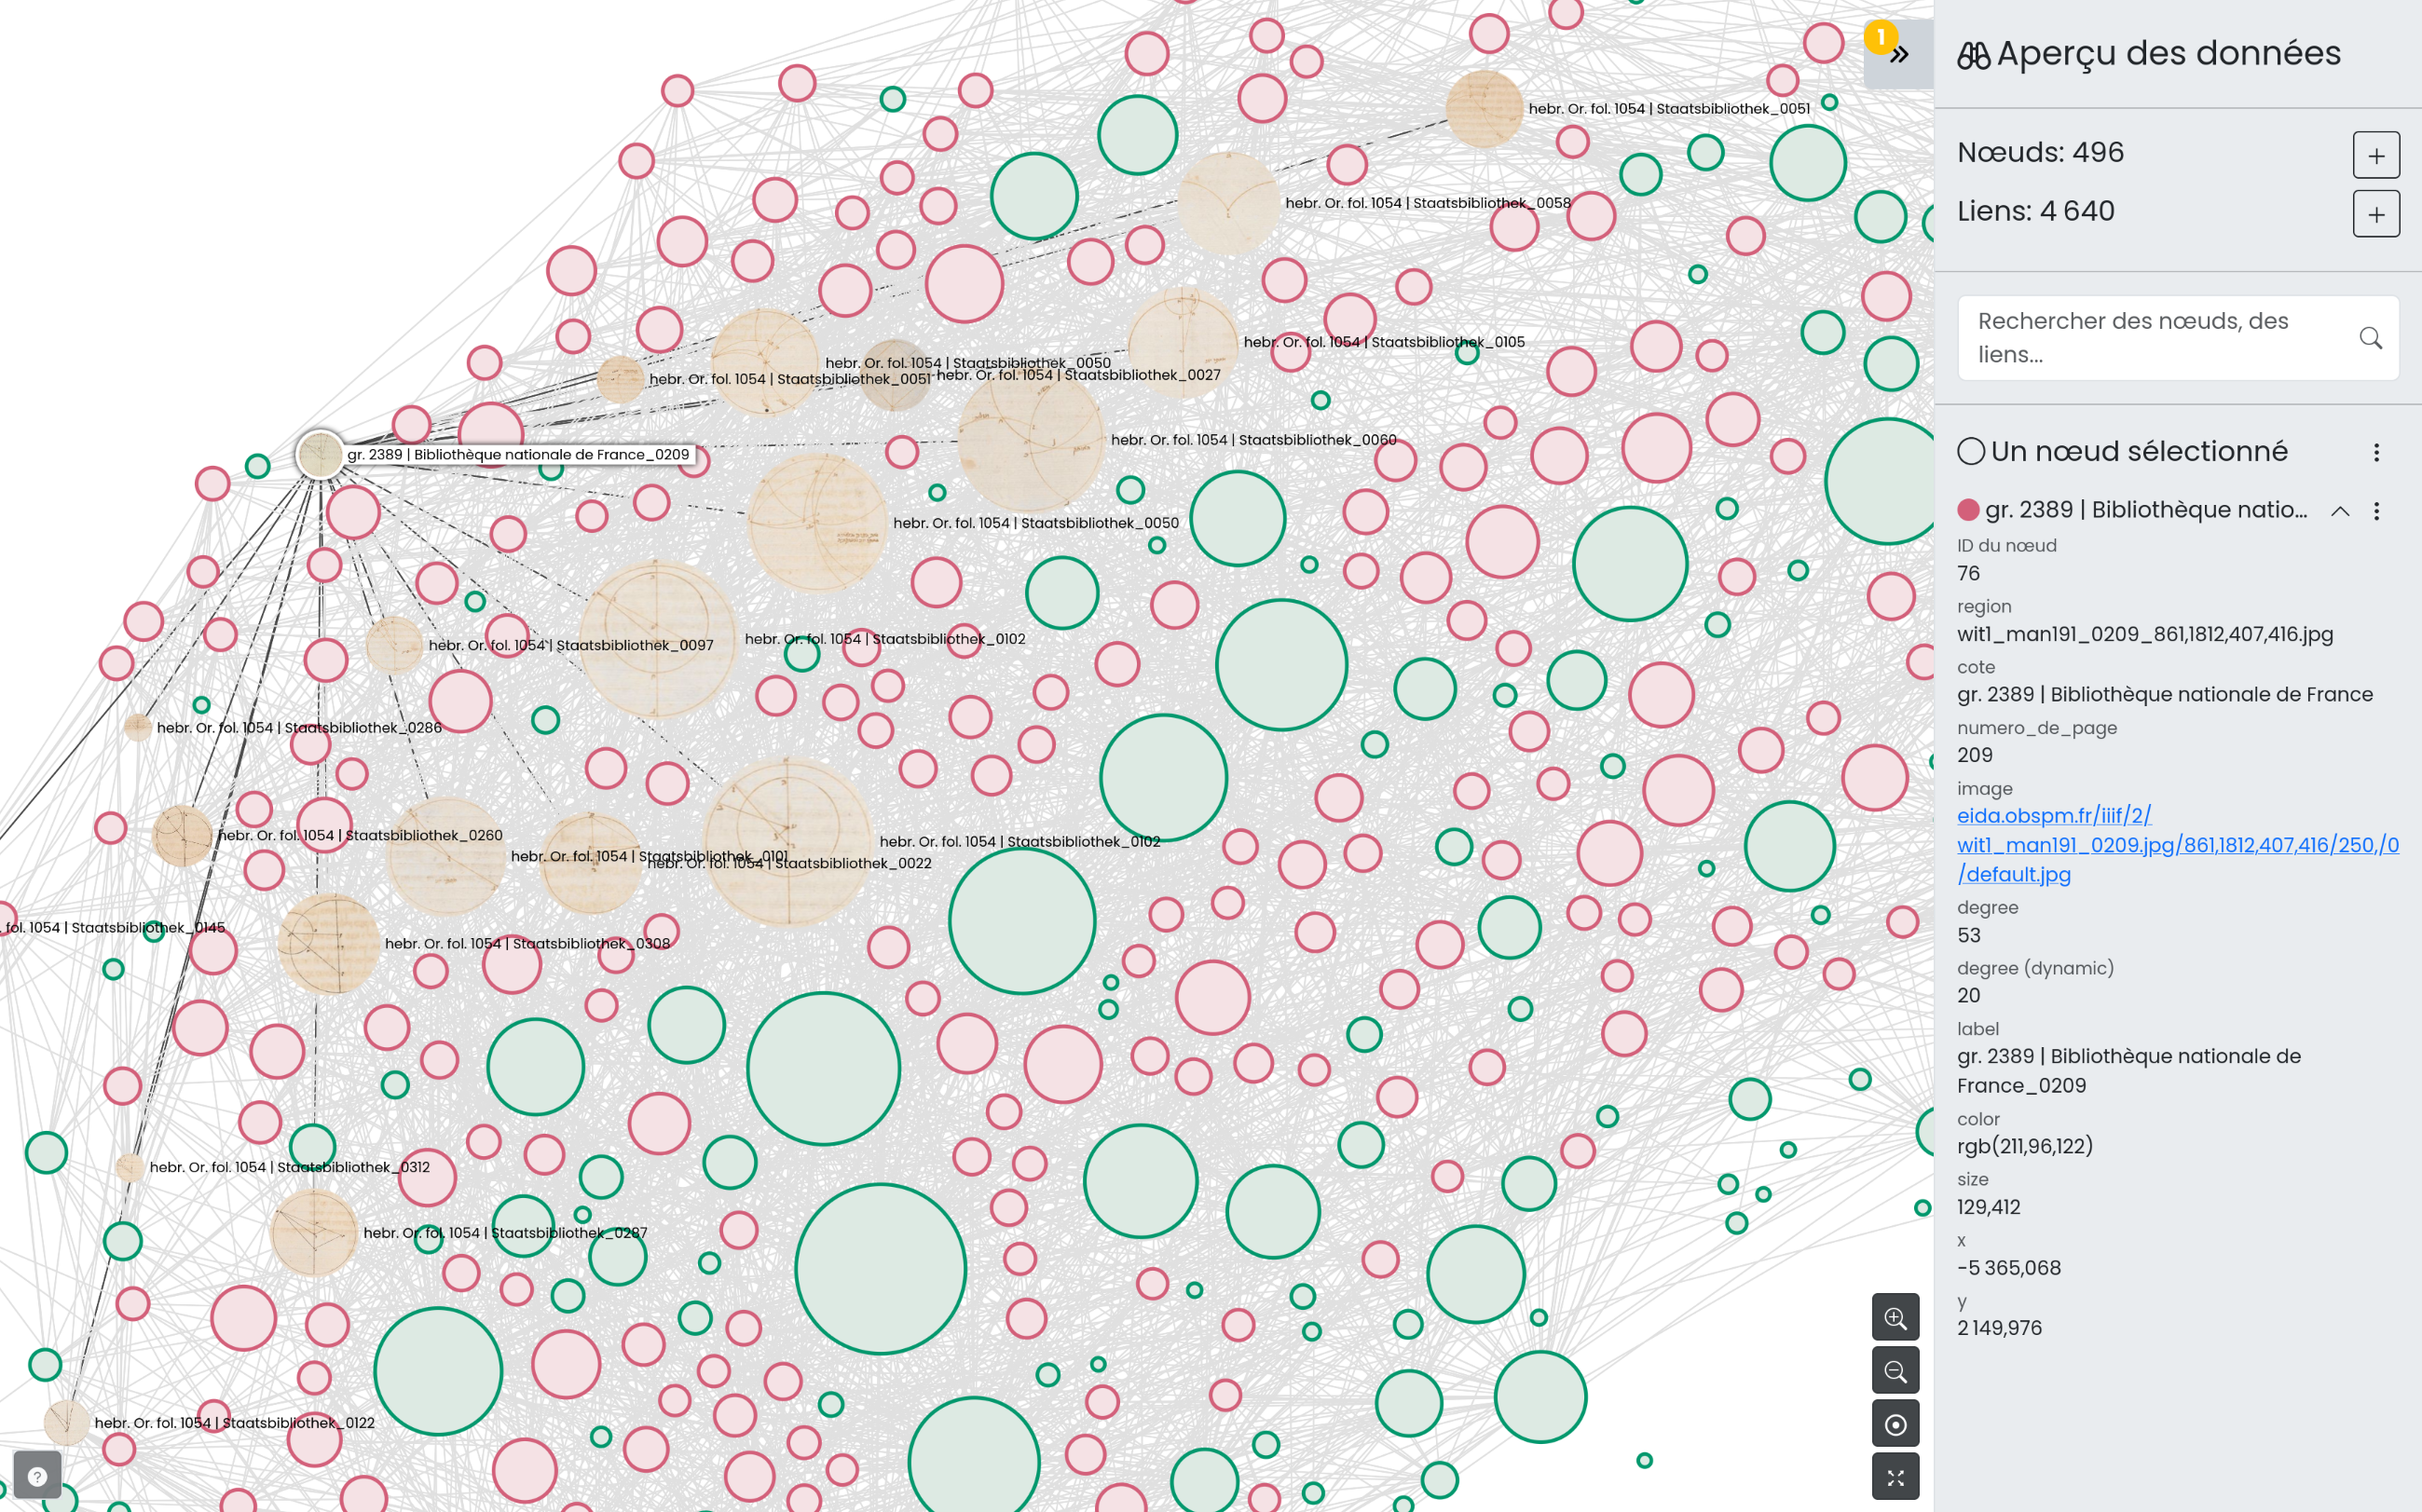
\includegraphics[width=0.8\textwidth]{images/apercu_force_directed_layout_1.png}
	\caption{Aperçu de la visualisation en \textit{force-directed layout}}
	\label{fig:forced_directed_1}
\end{figure}

Cette visualisation est composée de 496 nœuds et 4640 liens. Lorsque nous la regardons de plus près, nous notons un déséquilibre entre la taille des nœuds du \textit{witness 1} et ceux du \textit{witness 40}. En effet, ceux du manuscrit \textit{Grec 2389} ont tendance à être plus petits que ceux du \textit{Hebr. Or. fol 1054}. Il est important de signaler que les liens internes ont été supprimés au préalable pour rendre la visualisation plus lisible. Dans \textit{Hebr. Or. 1054}, certaines \textit{regions} correspondent à de nombreuses \textit{regions} similaires dans \textit{Grec 2389}, ce qui produit des concentrations visibles de liens vers quelques nœuds dans la visualisation. A l'inverse, pour le \textit{Grec 2389}, les \textit{regions} similaires sont plus dispersées, donc les liens partent vers des nœuds variés, ce qui donne une apparence plus éparse.

Les \textit{regions} contenues dans les nœuds plus conséquents du \textit{Hebr. Or. fol} reflètent les \textit{regions} qui présentent le plus grand nombre de similarités détectées automatiquement dans le \textit{Grec 2389}.

\begin{figure}[H]
	\centering
	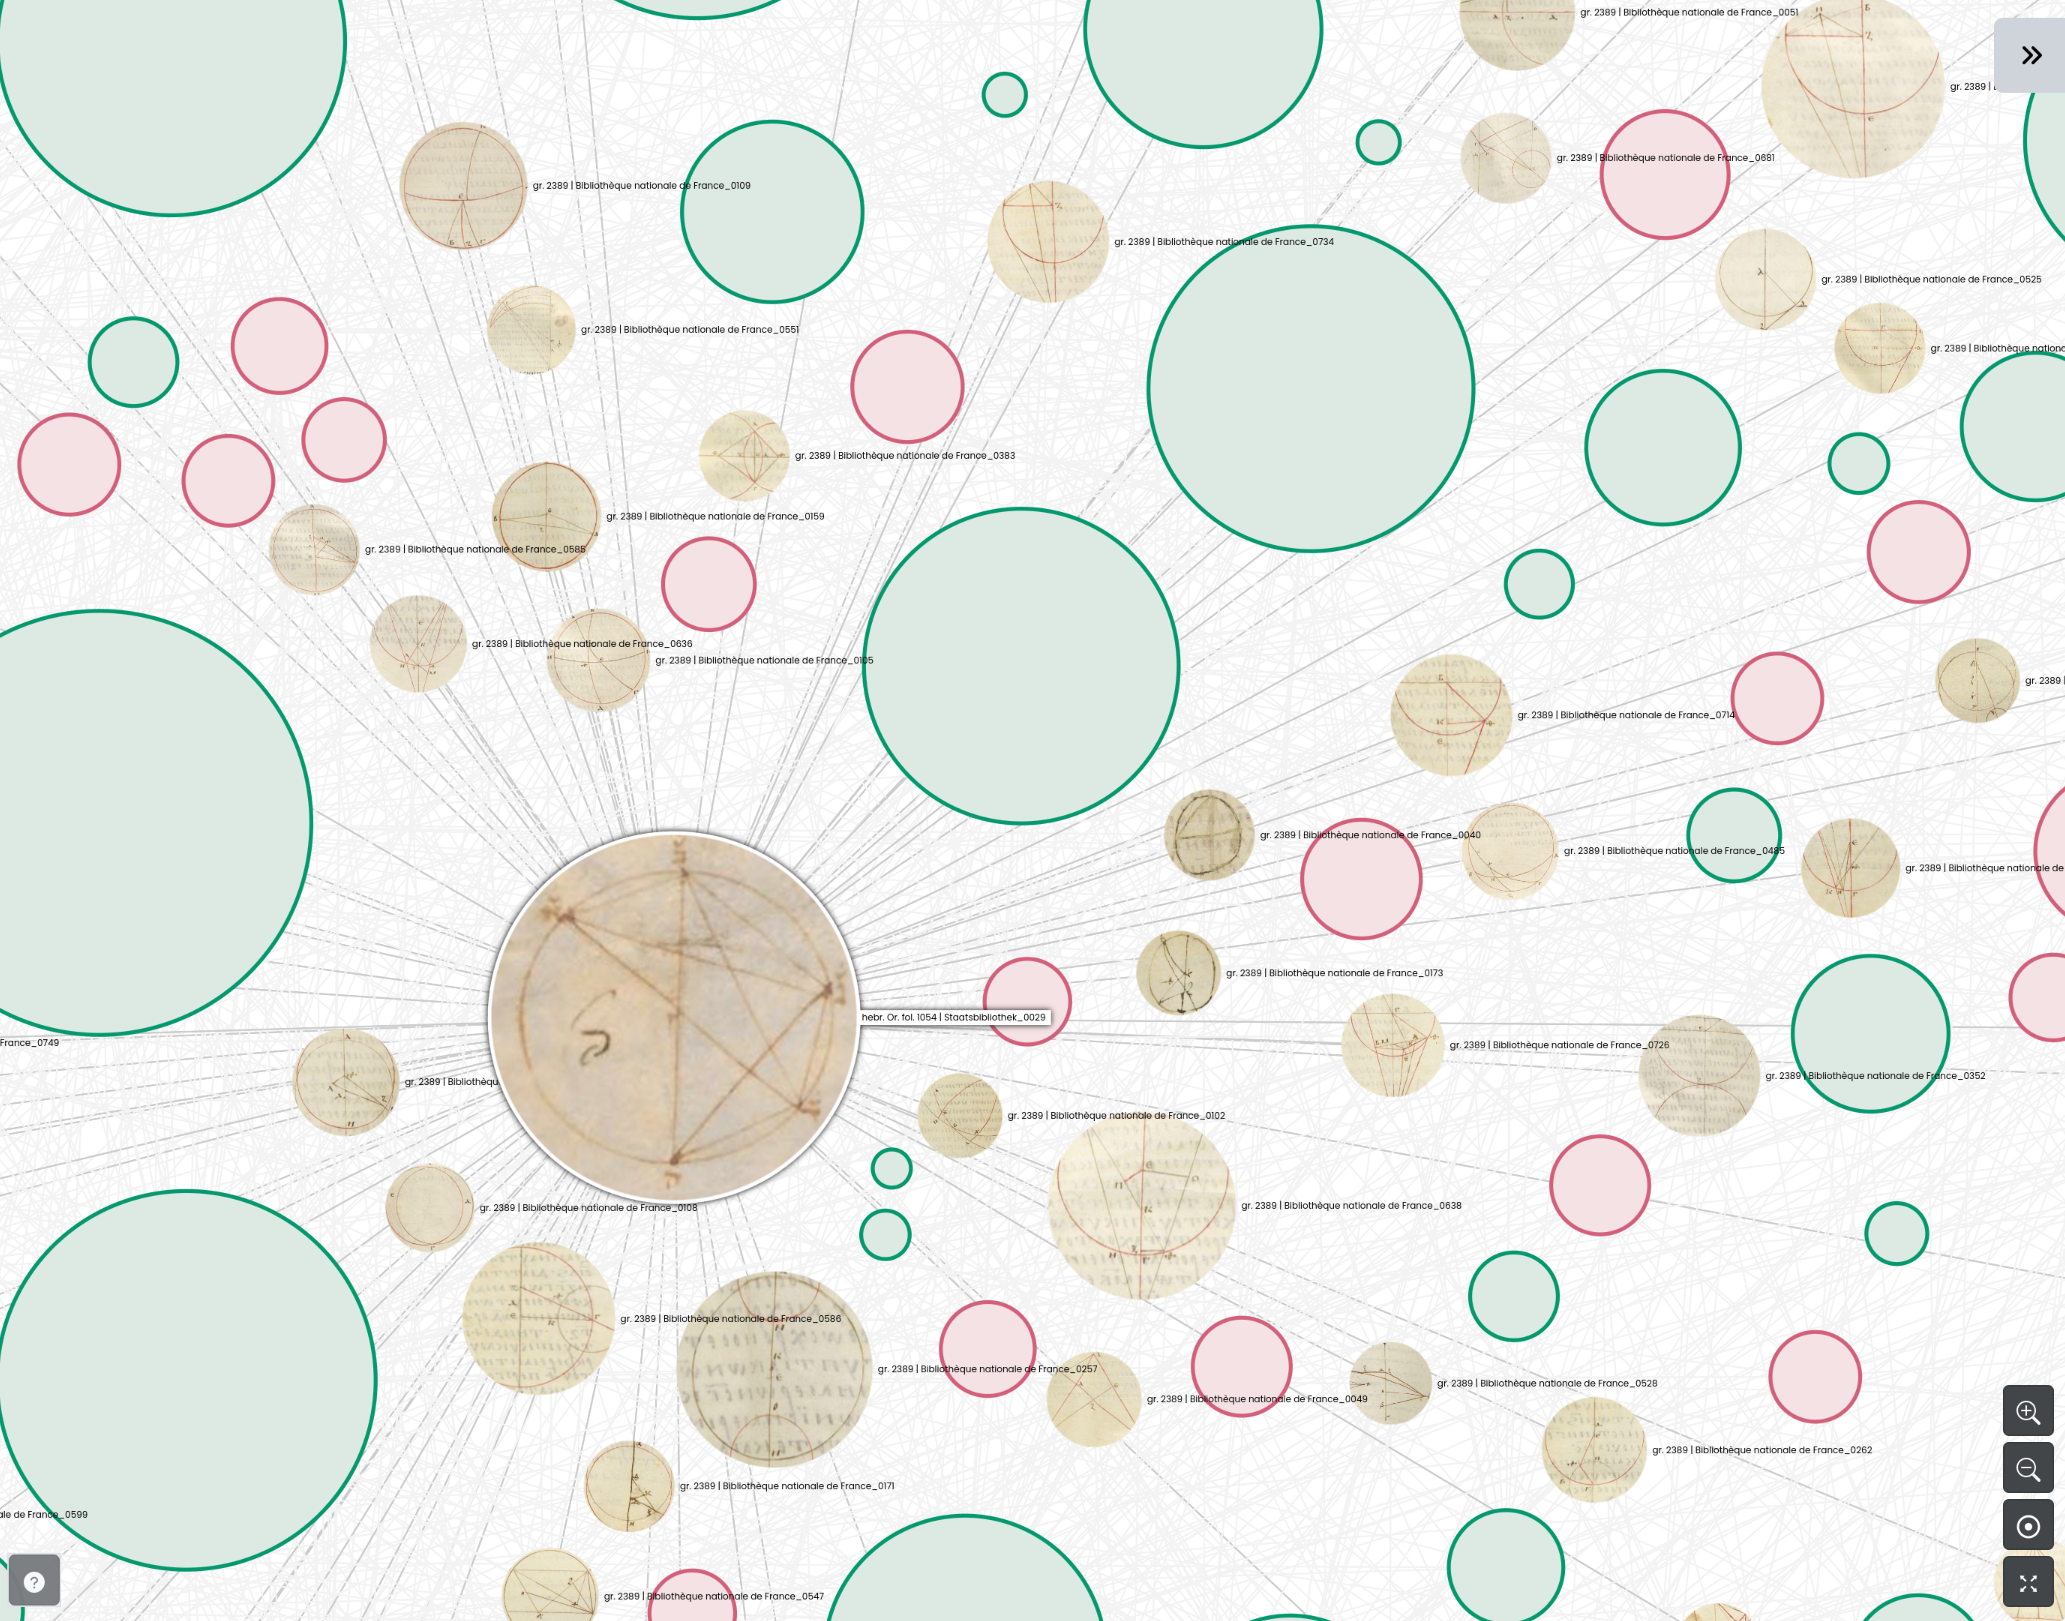
\includegraphics[width=1\textwidth]{images/apercu_force_directed_layout_2.png}
	\caption{Les résultats de la reconnaissance automatique de similarité restent approximatifs}
	\label{fig:forced_directed_2}
\end{figure}

Cependant, lorsque nous examinons les \textit{regions pairs} de plus près, nous nous rendons compte que beaucoup d'entre elles sont incorrectes. Il s'agit du principal défaut lié à la réalisation d'une visualisation à partir de données non vérifiées par les chercheurs après le traitement automatique. Il est donc difficile de tirer des conclusions à partir de cette dernière. Néanmoins, il est tout à fait envisageable d'utiliser cette visualisation avec des données annotées par les chercheurs. 